\chapter {Planificación}

\section{Metodología de desarrollo}
\begin{text}
	Todo proyecto software debe tener una organización y unas etapas de desarrollo bien definidas. En esta sección se pretende explicar la metodología de desarrollo elegida para realizar este proyecto. \\
	Se ha tratado como cualquier otro proyecto software. Para la organización y el control de versiones se ha elegido Github, un software basado en git originalmente creado para el control de versiones. \\
	En cuanto a la metodología de desarrollo, se ha optado por utilizar la metodología SCRUM. A continuación se explican con mayor detalle estos conceptos.
\end{text}

\subsection{¿Qué es un Milestone?}
\label{milestones}
\begin{text}
	Los milestones o hitos en castellano, corresponden con estados finales deseados de la aplicación. Sabiendo esto, podríamos crear un milestone por ejemplo: "Servidores configurados a través de ficheros de configuración Ansible". Esto será un estado final deseado para nuestra aplicación o proyecto. Para que un hito quede totalmente realizado, deben estar completos todos los issues marcados como esenciales para el hito. Un hito está compuesto por issues. A continuación se muestran algunos milestones creados en este proyecto, en el panel de administración GitHub.
	
	\clearpage
	
	\begin{figure}[!hbt]
		\centering
		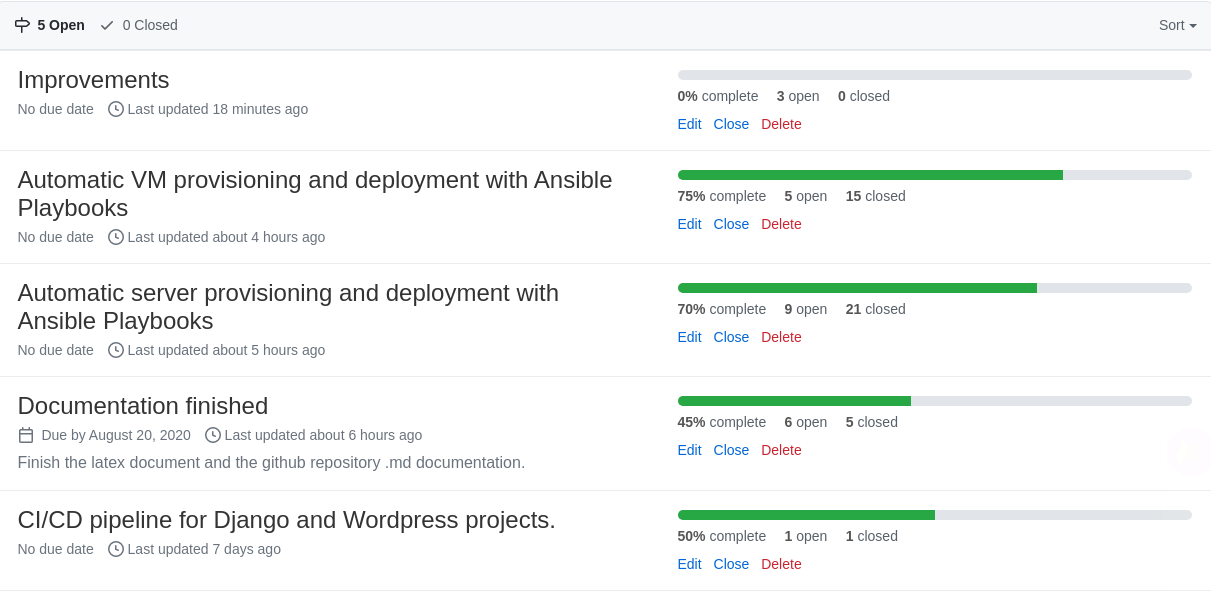
\includegraphics[scale=0.37]{imagenes/Analisis/milestones.png}
		\caption[GitHub milestones]{GitHub milestones \cite{github-issue}}
		\label{github_milestones}
	\end{figure}
\end{text}

\subsection{¿Qué es un Issue?}

\begin{text}
	Como ya hemos visto, los issues forman parte de los hitos. Es una forma de desgranar el problema. Siguiendo el ejemplo anterior, si tenemos un hito: "Servidores configurados a través de ficheros de configuración Ansible", podemos desgranar el siguiente en distintos issues, que serían tareas más sencillas que hay que realizar para completar el hito. Por ejemplo, algunos issues serían: 
	\begin{itemize}
		\item Crear estructura directorios Ansible.
		\item Instalar paquetes en servidor a través de ficheros de configuración Ansible. \textbf{Core}
		\item Configurar interfaces de red a través de ficheros de configuración Ansible. \textbf{Core}
		\item Instalar ISO en servidor a través de ficheros de configuración Ansible. \textbf{Core}
		\item Instalar certificados SSL a través de ficheros de configuración Ansible. \textbf{Mejora}
	\end{itemize}
	
	Y así seguiríamos creando issues según creamos que van a ser necesarios para completar el hito en cuestión. \\
	En la sección ``\nameref{milestones}'' hemos hablado que los issues tienen etiquetas. En la lista anterior por ejemplo, únicamente tenemos dos etiquetas que nos indican en este caso si son issues imprescindibles para el hito o simplemente mejoras. Gracias a estas etiquetas, podemos distinguir entre distintos tipos de issues y asignar mayor o menor prioridad por etiqueta. También gracias a Github, cada issue puede ser asignado a un desarrollador del proyecto. A continuación se muestra un ejemplo del panel de Github para mostrar los issues, etiquetas y hitos. \\
	Como se puede comprobar, el sistema de etiquetas y asignación de issues a desarrolladores, es más que suficiente para manejar proyectos. Permite asignar prioridades, agrupar issues en hitos y escribir comentarios en cada issue / milestone. 
	
\end{text}

\subsection{Milestones, Issues y SCRUM}
\begin{text}
	Como ya sabemos, SCRUM es una metodología de trabajo que permite agilizar la creación y la entrega del software. Pero, ¿Cómo encaja la metodología SCRUM en nuestra forma de trabajar con milestones e issues? Muy sencillo. Vamos a tratar cada milestone del proyecto como si fuese un sprint SCRUM y cada issue del proyecto como si fuese una tarea a asignar y realizar. Por lo tanto cada sprint finalizará con un MVP (Minimum Viable Product) y cuando se complete un sprint se pasará al siguiente.
	
	\begin{figure}[!hbt]
		\centering
		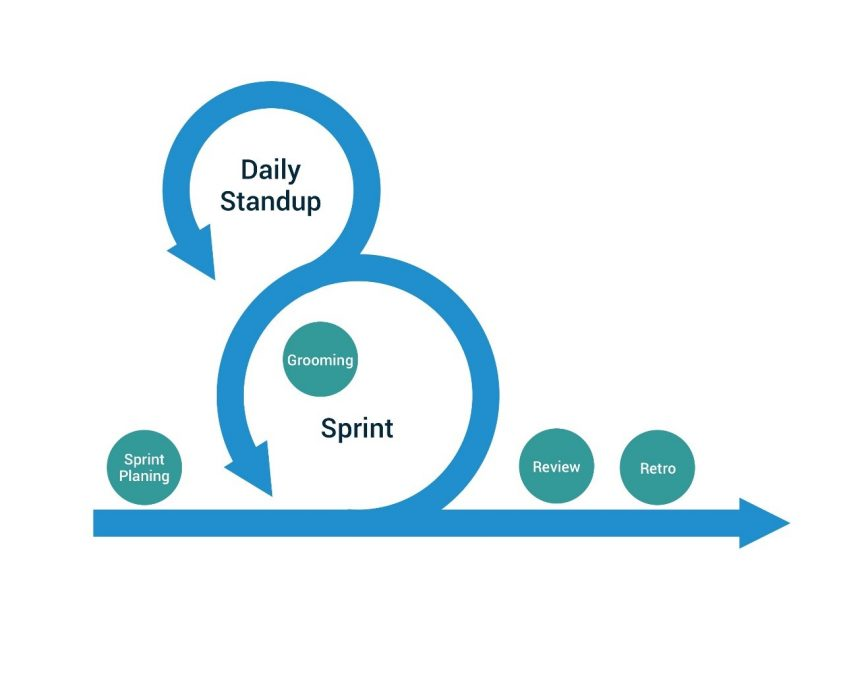
\includegraphics[scale=0.5]{imagenes/Planificacion/scrum.jpg}
		\caption[SCRUM]{SCRUM \cite{scrum:online}}
		\label{scrum_plan}
	\end{figure}
	\clearpage
	
	
	\begin{figure}[!hbt]
		\centering
		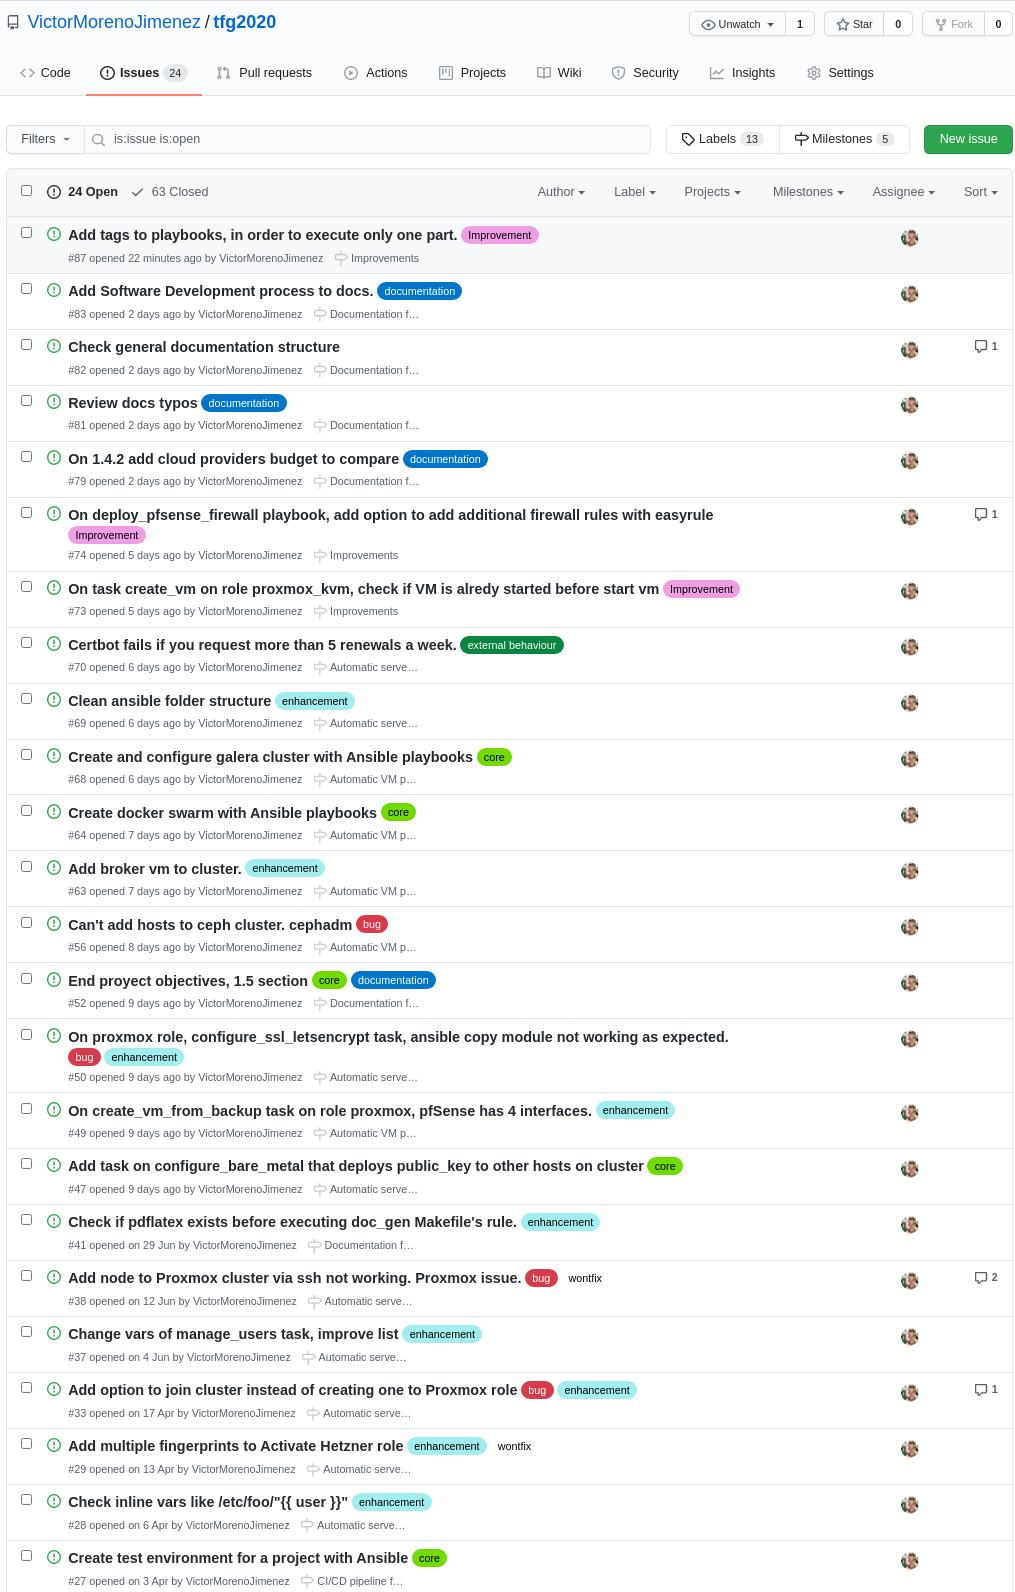
\includegraphics[scale=0.46]{imagenes/Analisis/githubissues.jpg}
		\caption[GitHub panel]{GitHub panel \cite{githubrepo:online}}
		\label{github_issues}
	\end{figure}
\end{text}
\clearpage

\section{Milestones e issues}
\begin{text}
	En el capítulo ``\nameref{capitulo1}'', se definen y detallan los objetivos que este proyecto pretende alcanzar. Sin embargo, estos objetivos presentan un alto grado de abstracción y es difícil trasladarlos a tareas concretas que se traducirán en issues del proyecto. Es por esto que en el capítulo ``\nameref{capitulo2}'' se desgranan estos objetivos en subobjetivos. En esta sección vamos a traducir los objetivos principales del proyecto en milestones, y traducir cada subobjetivo a un requisito funcional que se convertirá en un issue en el proyecto.
\end{text}

\subsection{Milestones}
\label{Milestones}
\begin{text}
	Los milestones son estados deseados del proyecto que queremos avanzar para completarlo. Cada milestone termina un MVP (Minimum Viable Product) y cubre las necesidades de algún objetivo. A continuación se definen los milestones y se agrupan por objetivos.
	
	\begin{itemize}
		\item \textbf{Milestone 0:}. Preparar entorno de desarrollo. Antes de comenzar el proyecto, se debe configurar el equipo que se va a utilizar para trabajar, instalando y configurando el software necesario. 
		\item \textbf{Milestone 1:} Servicio de virtualización desplegado. 
		\item \textbf{Milestone 2:} Firewall desplegado en cluster.
		\item \textbf{Milestone 3:} Control de versiones desplegado en cluster.
		\item \textbf{Milestone 4:} Cluster monitorizado.
		\item \textbf{Milestone 5:} Cluster preparado para desplegar aplicaciones.
		\item \textbf{Milestone 6:} Despliegue automático de aplicaciones.
	\end{itemize}
	A continuación se relaciona cada objetivo definido en la sección ``\nameref{objetivos_primarios}'' con su milestone.
	
	
	\begin{table}[!hbt]
		\begin{tabular}{llllll}
			& Objetivo1         & Objetivo2         & Objetivo3         & Objetivo4         & Objetivo5         \\
			Milestone1 & \textbf{X} & \textbf{X} & \textbf{}  &            &            \\
			Mliestone2 & \textbf{X} & \textbf{X} &            &            &            \\
			Milestone3 &            &            & \textbf{X} & \textbf{X} &            \\
			Milestone4 &            &            & \textbf{X} & \textbf{X} &            \\
			Milestone5 &            &            & X          & \textbf{X} &            \\
			Milestone6 &            &            &            &            & \textbf{X}
		\end{tabular}
	\end{table}
	
	Los milestones 1,2 están relacionados con la creación y replicación de la infraestructura base, mientras que los milestones 3,4 y 5 con los servicios desplegados en la infraestructura. milestone 6 asegura que existen cauces de integración continua y despliegue automático de aplicaciones.
	
\end{text}

\subsection{Issues}
\label{issues}
\begin{text}
	En esta subsección se van a redactar los issues necesarios para cumplir con los requisitos funcionales y agrupar estos issues en milestones. Los issues que mencionan la automatización de un servicio serán automatizados con la herramienta elegida en la sección ``\nameref{tecnologias_elegidas}''.
	
	\begin{itemize}
		\item \textbf{Milestone 0:} Entorno de desarrollo. 
		\begin{itemize}
			\item \textbf{Issue 0.1}. Crear playbooks de Ansible para configurar el equipo de desarrollo.
			\item \textbf{Issue 0.2} Crear playbooks de Ansible para crear la estructura de carpetas necesaria para el proyecto.
		\end{itemize}
		\item \textbf{Milestone 1:} Servicio de virtualización desplegado. 
		\begin{itemize}
			\item \textbf{Issue 1.1}. Automatizar instalación ISO en servidores Hetzner con rescue mode activado.
			\item \textbf{Issue 1.2}. Automatizar configuración LVM sobre ISO instalada.
			\item \textbf{Issue 1.3}. Automatizar instalación paquetes en los nodos.
			\item \textbf{Issue 1.4}. Automatizar gestión de usuarios/grupos del sistema en los nodos.
			\item \textbf{Issue 1.5}. Automatizar la instalación de servicio de virtualización Proxmox en los nodos.
			\item \textbf{Issue 1.6}. Automatizar gestión de usuarios/grupos Proxmox en los nodos.
			\item \textbf{Issue 1.7}. Automatizar gestión de almacenamiento Proxmox en los nodos.
			\item \textbf{Issue 1.8}. Automatizar creación e instalación certificado SSL en los nodos.
			\item \textbf{Issue 1.9}. Automatizar la creación del cluster Proxmox.
			\item \textbf{Issue 1.10}. Automatizar la adición de nuevos nodos al cluster.
		\end{itemize}
		\item \textbf{Milestone 2:} Firewall desplegado en cluster.
		\begin{itemize}
			\item \textbf{Issue 2.1}. Automatizar creación de máquina virtual pfSense en servicio de virtualización Proxmox.
			\item \textbf{Issue 2.2}. Modificar puerto SSH para poder ejecutar playbook sobre pfSense.
			\item \textbf{Issue 2.3}. Automatizar la configuración del firewall pfSense.
			\item \textbf{Issue 2.4}. Permitir la modificación de la configuración pfSense a través de un playbook de Ansible.
		\end{itemize}
		\item \textbf{Milestone 3:} Control de versiones desplegado en cluster.
		\begin{itemize}
			\item \textbf{Issue 3.1}. Automatizar la creación de máquina virtual en cluster donde instalar GitLab.
			\item \textbf{Issue 3.2}. Automatizar instalación GitLab en máquina virtual Proxmox.
			\item \textbf{Issue 3.3}. Automatizar configuración pfSense DHCP, añadir nueva IP.
			\item \textbf{Issue 3.4}. Automatizar configuración GitLab mediante ficheros de configuración.
		\end{itemize}
		\item \textbf{Milestone 4:} Cluster monitorizado.
		\begin{itemize}
			\item \textbf{Issue 4.1}. Automatizar la creación de máquina virtual en cluster donde instalar Icinga2.
			\item \textbf{Issue 4.2}. Automatizar instalación Icinga2 en máquina virtual Proxmox.
			\item \textbf{Issue 4.3}. Automatizar configuración pfSense DHCP, añadir nueva IP.
			\item \textbf{Issue 4.4}. Automatizar instalación Icinga2 Director sobre Icinga 2.
		\end{itemize}
		\item \textbf{Milestone 5:} Cluster preparado para desplegar aplicaciones.
		\begin{itemize}
			\item \textbf{Issue 5.1}. Automatizar instalación y configuración de Ceph cluster.
			\item \textbf{Issue 5.2}. Automatizar instalación y configuración der Galera cluster.
			\item \textbf{Issue 5.3}. Automatizar instalación y configuración de Virtualmin.
			\item \textbf{Issue 5.4}. Automatizar instalación y configuración de Kubernetes cluster.
			\item \textbf{Issue 5.5}. Automatizar instalación y configuración de RabbitMQ.
			\item \textbf{Issue 5.6}. Automatizar instalación y configuración de Nginx.
			\item \textbf{Issue 5.7}. Automatizar instalación y configuración de servicio orquestador de contenedores.
		\end{itemize}
		\item \textbf{Milestone 6:} Despliegue automático de aplicaciones.
		\begin{itemize}
			\item \textbf{Issue 6.1}. Dockerizar proyecto Django + Angular.
			\item \textbf{Issue 6.2}. Instalación y configuración de GiLab CI+CD.
			\item \textbf{Issue 6.3}. Adaptar proyecto a CI/CD.
		\end{itemize}
	\end{itemize}
\end{text}

\section{Estimación recursos necesarios}
\begin{text}
        En esta sección se va a crear una estimación de los recursos, tanto humanos como económicos que se van a necesitar para llevar a cabo el proyecto. Cabe destacar que en la estimación temporal se incluye un lapso de tiempo para adaptarse a la tecnología a usar. Esto no se ha indicado de forma explícita, pero va implícito en estimación temporal de ejecución de cada hito. \\ 

\end{text}
\subsection{Estimación temporal}
\begin{text}
        Para dar una estimación del tiempo requerido para el proyecto, vamos a utilizar un diagrama de Gantt, en el que incluiremos los principales hitos del proyecto y una estimación en semanas de la duración del mismo. Una estimación inicial ha sido de 23 semanas en total. Cabe destacar que se ha utilizado la metodología de desarrollo SCRUM, cada uno de los hitos se ha traducido en un sprint. Cada hito ofrece un MVP (Minimum Viable Product) con unas funcionalidades bien definidas. Ver la seccción ``\nameref{Milestones}''. A continuación se muestra el diagrama de Gantt con la planificación pensaba para este proyecto. Se ha pensado este diagrama para una jornada de trabajo de 5 horas diarias 5 días a la semana, es decir una jornada de 25 horas semanales.
\end{text}

\newpage
\subsubsection{Diagrama Gantt}
        \begin{figure}[!hbt]
                \centering
                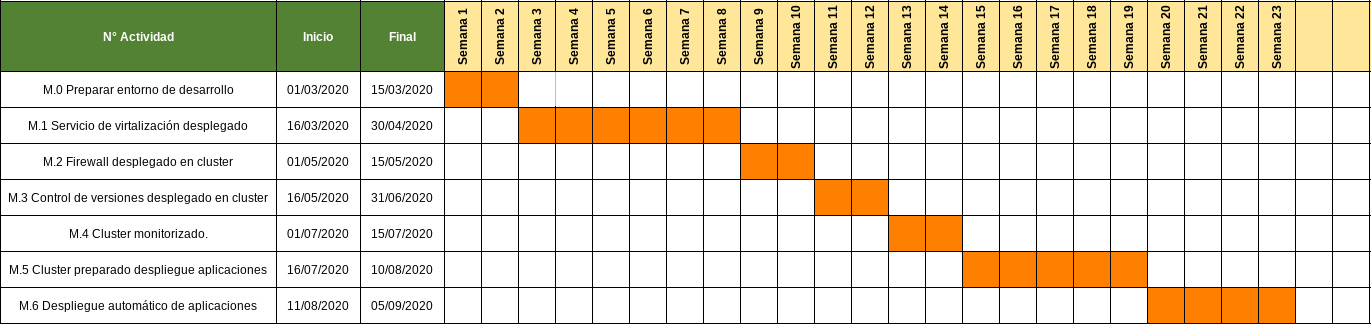
\includegraphics[scale=0.4,angle=-90]{imagenes/Planificacion/gannt2.png}
                \caption[Diagrama Gantt]{Diagrama Gantt \cite{Gantt:online}} 
                \label{Diagrama Gannt}
        \end{figure}
\clearpage
\subsection{Presupuesto}
\label{presupuesto}
        \begin{text}
            Para realizar este presupuesto, se ha partido del sueldo base de un graduado en Ingeniería Informática. Recalcar que en esta partida, se incluyen horas extra para formación en las tecnologías elegidas. Este presupuesto es lo que costaría el desarrollo del proyecto.
            Por otra parte se ha incluido en el presupuesto el coste de mantenimiento de la infraestructura.
        \end{text}
        \\
        \begin{table}[ht]
                \centering
                \begin{tabular}[!hbt]{SSSSSSSS} \toprule
                        {Concepto} &  {Precio / mes \euro} & {Importe Total \euro} \\ \midrule
                        {\textbf{Partida Personal}} \\ \midrule
                        {Sueldo DevOps Junior}  & {1.800} & {3.600}  \\
                    \midrule
                        {\textbf{Partida Inventariable}} \\ \midrule
                        {Coste infraestructura}  & {61,34}  & {368,04}   \\
                        \midrule
                        {\textbf{Partida Fungible}} \\ \midrule
                        {-}  & {-}  & {-}   \\
                        \midrule
                        {\textbf{Partida servicios técnicos}} \\ \midrule
                        {Mantenimiento}  & {Incluido}  & {0} \\
                        \midrule
                        {\textbf{Partida viajes y dietas}} \\ \midrule
                        {-}  & {-}  & {-} \\
                        \midrule
                        {\textbf{Partida de otros}} \\ \midrule
                        {Incluido}  & {Incluido}  & {0} \\
                        \midrule
                        {\textbf{Total}}  & {1861,34 \euro}  & {3.968,04 \euro} \\
                        \\ \midrule
                 \\ \bottomrule
                \end{tabular}
                \caption[Presupuesto]{Presupuesto \cite{presupuesto:online}} 
                \label{Presupuesto}
        \end{table}

        \begin{text}
                Cabe destacar que en esta partida únicamente se incluyen el coste de un empleado Junior y el coste de la infraestructura necesaria para desarrollar este proyecto. Nótese que en ningún caso, se están añadiendo costes de oficina ni de equipo para desarrollo. En una partida real, habría que incluir estos gastos ya que son imprescindibles para el proceso de desarrollo. En este presupuesto aparece como Otros.
        \end{text}